\documentclass{resume}

\begin{document}

\fontfamily{ppl}\selectfont

\noindent
\begin{tabularx}{\linewidth}{@{}m{0.8\textwidth} m{0.2\textwidth}@{}}
{
    \Large{Andrés Fuentes Hernández} \newline
    \small{
        \clink{
            \href{mailto:andres7233@hotmail.com}{andres7233@hotmail.com} \textbf{·} 
            {\fontdimen2\font=0.75 55 5287 9324} 
            \par
            \href{https://www.linkedin.com/in/andrés-fuentes-bbb78188/}{https://www.linkedin.com/in/andrés-fuentes-bbb78188}
        } \newline
    }
} & 
{
    \hfill
    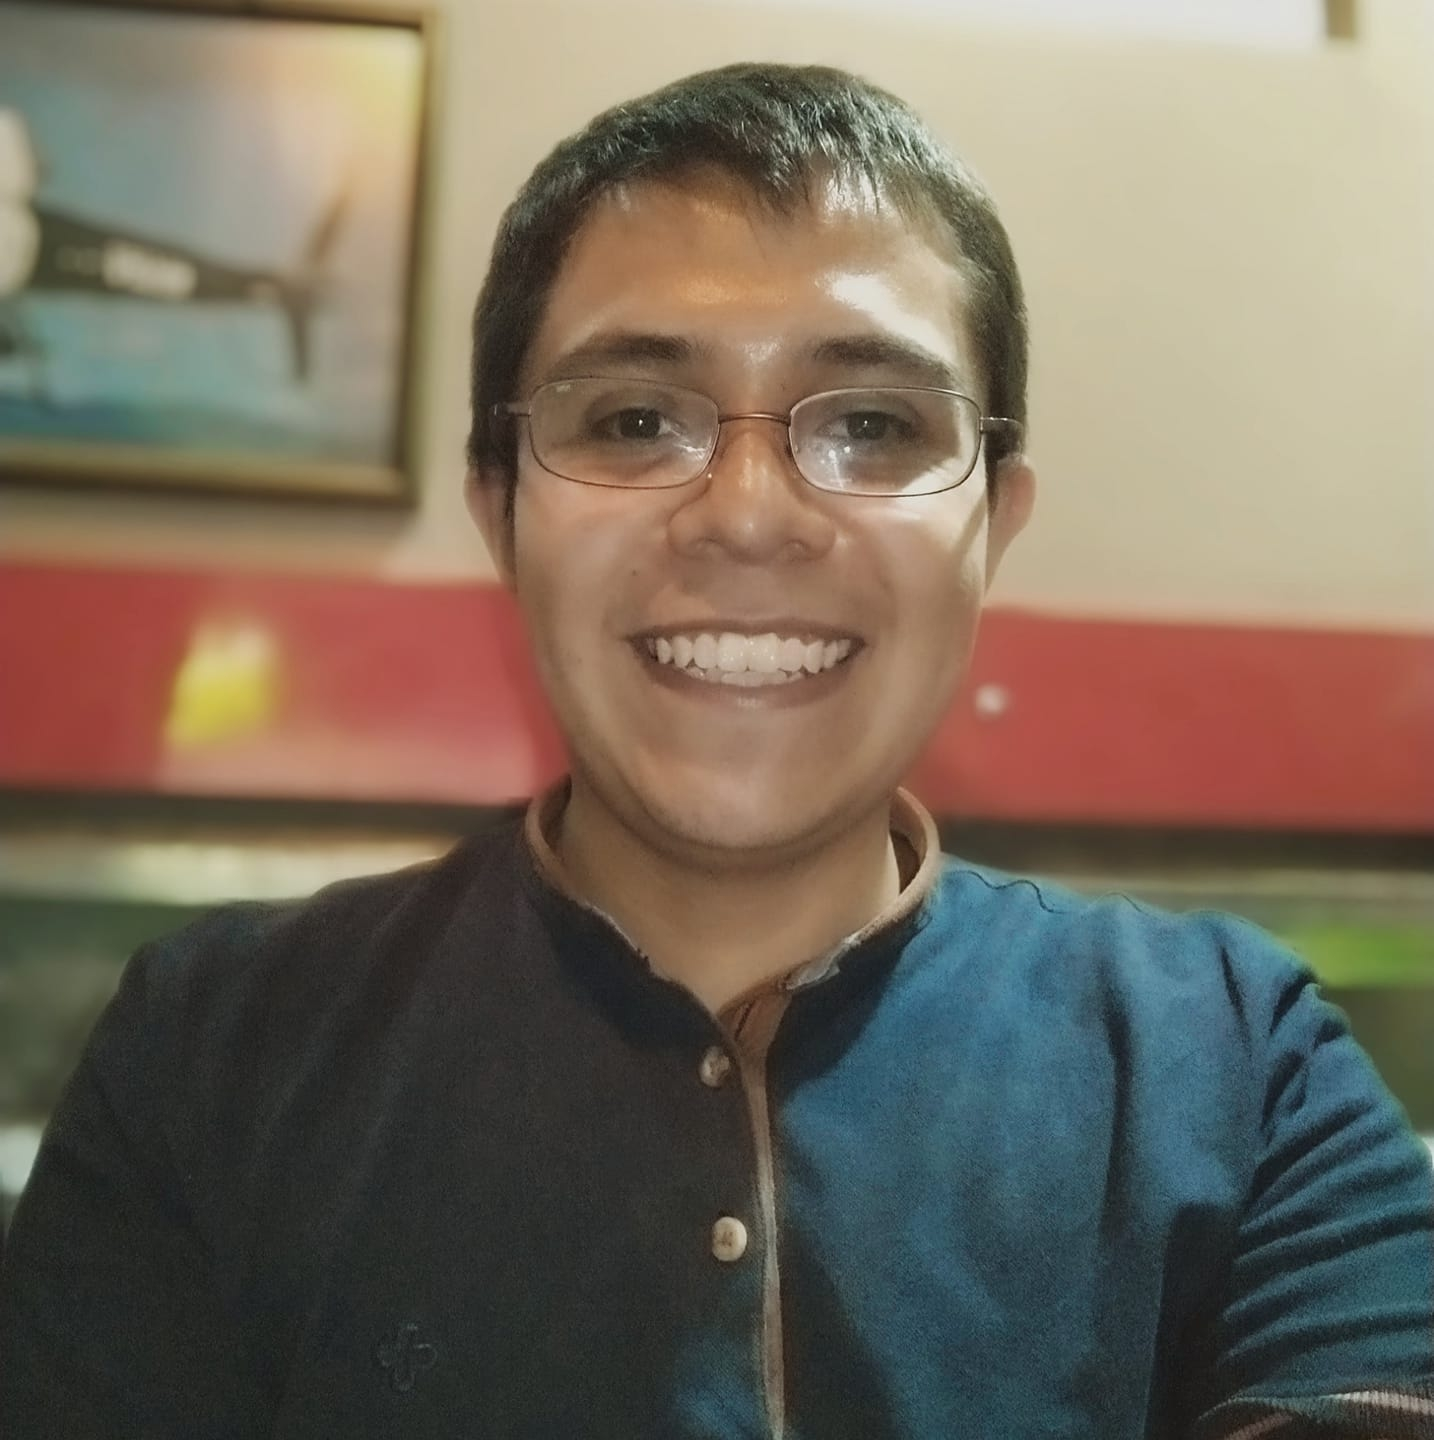
\includegraphics[width=2.8cm]{images/foto.jpg}
}
\end{tabularx}

\begin{center}
\begin{tabularx}{\linewidth}{@{}*{2}{X}@{}}{
    \psection{PROFILE}{\footnotesize
    Software developer with a 4 year experience in back-end development. I love learning all kind of things and teaching what I know, that is why I chose to be  a software engineer, because there are always recent technologies to learn, new business rules to understand and new teammates to work with. Finally I can say that I consider that my biggest asset is my curiosity.
    }
}
\end{tabularx}
\begin{tabularx}{\linewidth}{@{}*{2}{X}@{}}
% left side %
{
    \csection{EXPERIENCE}{\small
        \begin{itemize}
            % item 1 %
            \item \frcontentDate{Skytouch technology}{Software Engineer - Remote}{ August 2019 - Current}{Implantation and design of multiple flows for a management system platform for hotels, migration from monolith to micro-services using AWS.}
            
            % item 2 %
            \item \frcontentDate{Sngular México}{Junior software Engineer − México}{August 2017 - August 2018}{Worked as a contractor for a bank, developing front-end and back-end projects on its platform for small businesses.}
            
            \item \frcontentDate{Code Ingeniería}{Junior software Engineer − México}{June 2016 - August 2017}{Worked on a government project in which I had the accountability of production environment maintenance and deployments, attended service calls and developed new features into the system. When the company grew I was in charge of mentoring new developers into the inner workings of the system.}

        \end{itemize}
    }
    \csection{COURSES \& CERTIFICATIONS }{\small
        \begin{itemize}
            % item 1 %
            \item \frcontent{Oracle Certified Associate Java 8}{}{Oracle}{2018}
        \end{itemize}
    }
} 
% end left side %
& 
% right side %
{
    \csection{EDUCATION}{\small
        \begin{itemize}
            % item 1 %
            \item \frcontent{M.Sc. Computer Science}{IIMAS-UNAM}{}{August 2019 - Current}
            \item \frcontent{B.S. Bionic engineering}{UPIITA-IPN}{}{August 2009 - January 2016}
            \item \frcontent{Digital systems Technician}{Vocacional 9-IPN}{}{August 2006 - June 2009)}
        \end{itemize}
    }
    \csection{SKILLS}{\small
        \begin{itemize}
            \item \textbf{Programming languages \& Technologies} \newline
            {\footnotesize Java, Golang, C, SQL, javascript, HTML, CSS, AWS, Spring boot, Microsoft SQL server, MySQL, liquidbase, JUnit, Power Mock, Maven, Git}{}{}
            \item \textbf{Patterns \& Practices} \newline
            {\footnotesize Object Oriented Programming, Functional  Programming, Unit testing, Microservices, Design patterns, Anti patterns}
            \item \textbf{Project Management methodologies \& platforms} \newline
            {\footnotesize Scrum, Jira}
            \item \textbf{Languages} \newline
            {\footnotesize English, Spanish}
        \end{itemize}
    }
    %\csection{OTHER HIGHLIGHTS}{\small
    %%    \begin{itemize}
    %%        \item {\footnotesize Gave talk on \textit{Achieving Rapid Response Times in Large Online Services} at Berkeley AMPLab Cloud.}
    %%        \item {\footnotesize Led several teams across infrastructure, founded \textit{Google Brain} and was involved in hiring process.}
    %%    \end{itemize}
    %%}
    %%\csection{HOBBIES \& INTERESTS}{\small
    %%    \vspace{0.32cm}
    %%    \begin{tabularx}{\linewidth}{@{}*{4}{>{\centering\arraybackslash}X}@{}}
    %%        {\centering
    %%        
\includegraphics[width=0.8cm]{images/userexperience.png}
    %%        } &
    %%        {\centering
    %%        
\includegraphics[width=0.8cm]{images/lamp.png}
    %%        } & 
    %%        {\centering
    %%        
\includegraphics[width=0.8cm]{images/healthcare.png}
    %%        } &
    %%        {\centering
    %%        
\includegraphics[width=0.8cm]{images/cauldron.png}
    %%        } \\
    %%        {\footnotesize UI/UX} & {\footnotesize Problem Solving} & {\footnotesize Healthcare} & {\footnotesize Open Source}
    %%    \end{tabularx}
    %%}
}
\end{tabularx}
\end{center}
\end{document}